\subsection{Ethylene combustion in a perfectly stirred reactor}
The PSR model of Omnisoot\footnote{\href{https://github.com/mohammadadib-cu/omnisoot-cv/tree/main/examples/psr_pfr}{https://github.com/mohammadadib-cu/omnisoot-cv/tree/main/examples/psr\_pfr}} was used to simulate ethylene combustion at different equivalence ratios, $\phi = 1.9$, 2.0, and 2.1 in a perfectly stirred reactor connected to a flow reactor~\citep{manzello2007soot}. PSD measurements were conducted at the end of the flow reactor using a Nano-Differential Mobility Analyzer (Nano-DMA). The volume and nominal residence time of the PSR are 250~ml and 11~ms, respectively~\citep{manzello2007soot}. The flow reactor is 70~cm long with an inner diameter of 5.1~cm. The reactants are assumed to enter the adiabatic PSR at 300~K with an inlet mass flow rate of $\dot{m}_{in} = \rho V / \tau$, where $\rho$ was calculated at the reactor temperature of 1723~K~\citep{lenhert2009effects}. The PSR simulation was continued until a steady-state condition was reached for all the solution variables. The final gas composition, temperature, and soot properties from the PSR were used as inlet conditions for the PFR simulations, which yielded an average axial velocity of 14.5~m/s in the PFR, which is consistent with the values reported by~\citet{manzello2007soot}.

The KAUST mechanism was used to describe the gas-phase chemistry. The inception and PAH adsorption adjustment factors were varied for each PAH growth model to match the predicted PSD with the measurements as closely as possible for all three equivalence ratios. As shown in Figure~\ref{fig:psrpfr_psd}, all inception models capture the peak number concentration and the unimodal shape of the PSD, indicating that particle inception has ceased and coagulation is the dominant mechanism for agglomerate size growth. As reported in Table~\ref{tab:psrpfr_morpcomp}, the geometric mean mobility diameter, $d_{m,g}$, and the geometric mobility standard deviation, $\sigma_{m,g}$, obtained using all inception models are in good agreement with the values calculated from the measured PSD~\citep{manzello2007soot}. As shown in Figures~\ref{fig:psrpfr_psd}a and~\ref{fig:psrpfr_psd}b, the spread of the predicted PSD is narrower than that of the measurements for $\phi = 1.9$ and 2.0, corresponding to an underprediction of $\sigma_{m,g}$ for these equivalence ratios.



\begin{figure}[H]
	\centering
	\begin{tikzpicture}
		\draw (0, 0) node[inner sep=0] 	{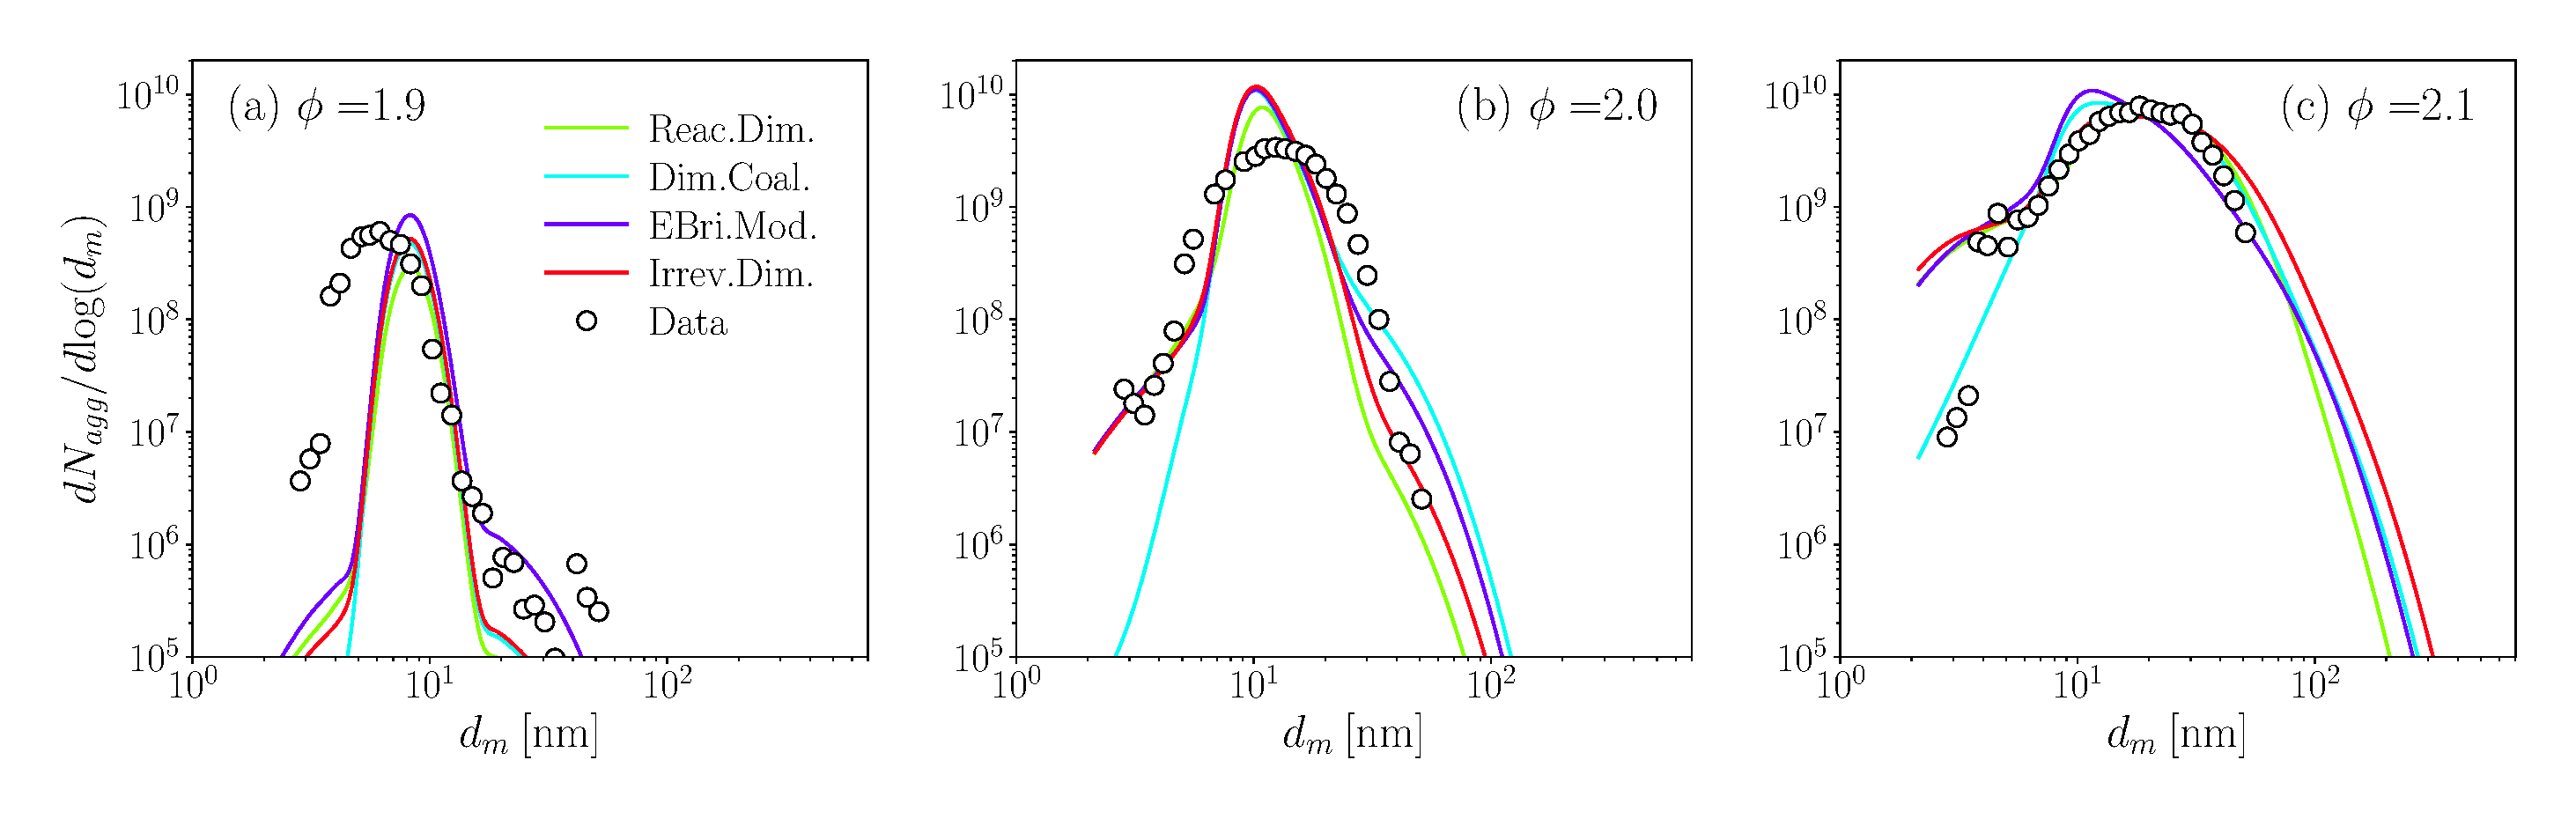
\includegraphics[width=1\textwidth]{Figures/Results/PSR/PSD_eq_ratio_log.pdf}};
		\draw (-3.05, 0.55) node {\tiny{\cite{manzello2007soot}}};
		%\draw (1.95, 0.66) node {\tiny{\cite{manzello2007soot}}};
		%\draw (5.5, -1.28) node {\tiny{\cite{manzello2007soot}}};
	\end{tikzpicture}
	\caption{The particle size distribution at the end of PFR for $\phi=1.9$ (a), 2.0 (b), and 2.1 (c) obtained using KAUST mechanism, SPBM and different inception models calibrated to match the predictions with the PSD measurements~\citep{manzello2007soot}.}
	\label{fig:psrpfr_psd} 
\end{figure}

All inception models underpredict the number concentration of small particles ($d_m < 6$~nm) at $\phi = 1.9$. The discrepancy decreases at $\phi = 2.0$, and the model predictions align well with the measurements. In the simulation results, the number concentration of the smallest particles with a diameter of 2~nm is strongly affected by the equivalence ratio, as the precursor production rate increases with $\phi$. This behavior can be better understood by comparing the acenaphthylene (A2R5) mole fraction at different $\phi$ values, as shown in Figures~\ref{fig:psrpfr_Iinc_PAH}a-c. The inlet mole fraction of A2R5 at $z = 0$~m corresponds to the value obtained from the PSR, which increases by factors of 10 and 4 when $\phi$ is increased incrementally from 1.9 to 2.0, and from 2.0 to 2.1, respectively. This relative increase is nearly the same across all inception models. As shown in Figures~\ref{fig:psrpfr_Iinc_PAH}d-e, the jump in A2R5 mole fraction leads to a substantial increase in the inception flux, which explains the sensitivity of the smallest particle concentrations to the equivalence ratio. The strong similarity between the A2R5 mole fraction profiles and the soot inception profiles along the reactor highlights the dominant role of A2R5 in soot inception. Another important observation is that the A2R5 mole fraction is not affected by the choice of inception model.


%All inception models underpredict the number concentration of small particles ($d_m<6$ nm) at $\phi=1.9$. The discrepancy decreases for $\phi=2.0$ and the model predictions align well with the measurements. In the simulation results, the number concentration of the smallest particles with the diameter of 2 nm is strongly affected by equivalence ratio because the precursor production rate increases with $\phi$. This can be better understood by comparing acenaphthylene (A2R5) mole fraction for different $\phi$ values shown in Figure~\ref{fig:psrpfr_Iinc_PAH}a-c. The inlet mole fraction of A2R5 at $z=0$ m corresponds to the mole fraction obtained by PSR, which increases by a factor of 10 and 4 when $\phi$ incrementally increase from 1.9 to 2.0, and 2.0 to 2.1, respectively. This relative increase is nearly the same for all inception models. As shown in Figure~\ref{fig:psrpfr_Iinc_PAH}d-e, the jump in A2R5 mole fraction causes a larger increase inception flux that justifies the sensitivity of the smallest particles to equivalence ratio. The strong similarity of profiles of A2R5 mole fraction and soot inception along the reactor shown highlights the dominant role of A2R5 chemistry on soot inception. Another important observation is that A2R5 mole fraction is not affected by the employed inception model.

As shown in Figure~\ref{fig:psrpfr_dp}, $d_p$ along the PFR is nearly identical for all inception models at $\phi = 1.9$, but the differences become more noticeable at higher $\phi$ values. The Reactive Dimerization model predicts the largest final $d_p$ because it channels more PAH mass into surface growth rather than inception, which is consistent with the lower peak number concentration observed in Figure~\ref{fig:psrpfr_psd}. The value of $d_p$ decreases rapidly at the beginning of the reactor due to a surge in the production of incipient particles (spherical particles with a diameter of 2~nm), which lowers the mean $d_p$. It then increases toward the end of the reactor as surface growth becomes dominant. Although the final $d_p$ increases slightly with $\phi$, the overall range remains similar across $\phi$ values, indicating a comparable balance between inception and surface growth. 

As shown in Figure~\ref{fig:psrpfr_fv}, the soot volume fraction, however, is highly sensitive to $\phi$, which can be attributed to the strong influence of $\phi$ on precursor production, inception flux, and the number of particles. An analysis of surface growth rates at the end of the PFR revealed that more than 95\% of the soot mass is acquired through the HACA mechanism. Figure~\ref{fig:psrpfr_Nagg_HACA} illustrates the coupling between $N_{agg}$ and the HACA growth rate, and how both respond to changes in $\phi$.


%As shown in Figure~\ref{fig:psrpfr_dp}, $d_p$ along the flow reactor is nearly the same for all inception models at $\phi=1.9$, but the difference becomes noticeable for higher $\phi$ values. Reactive Dimerization model predicts the largest final $d_p$ because it directs more PAH mass to surface growth rather than inception, which is consistent with lower peak number concentration observed in Figure~\ref{fig:psrpfr_psd}. $d_p$ rapidly decreases at the beginning of the reactor flow due to the rise in the production of incipient particles (spherical particles with diameter of 2 nm) that lowers the mean $d_p$ of particles. Then, $d_p$ increases by surface growth towards the end of reactor. The final $d_p$ slightly increases with $\phi$, but its range is similar for $\phi$ values indicating a similar inception to surface growth balance. As shown in Figure~\ref{fig:psrpfr_fv}, soot volume fraction, however, is very sensitive to $\phi$, which can be explained by the strong effect of $\phi$ on precursor production, inception flux, and number of particles. The analysis of surface growth rates at end of PFR revealed that more than 95\% of soot mass is gained through HACA. Figure~\ref{fig:psrpfr_Nagg_HACA} illustrates the coupling between $N_{agg}$ and HACA growth rate and their change due to $\phi$.  


\begin{figure}[H]
	\centering
	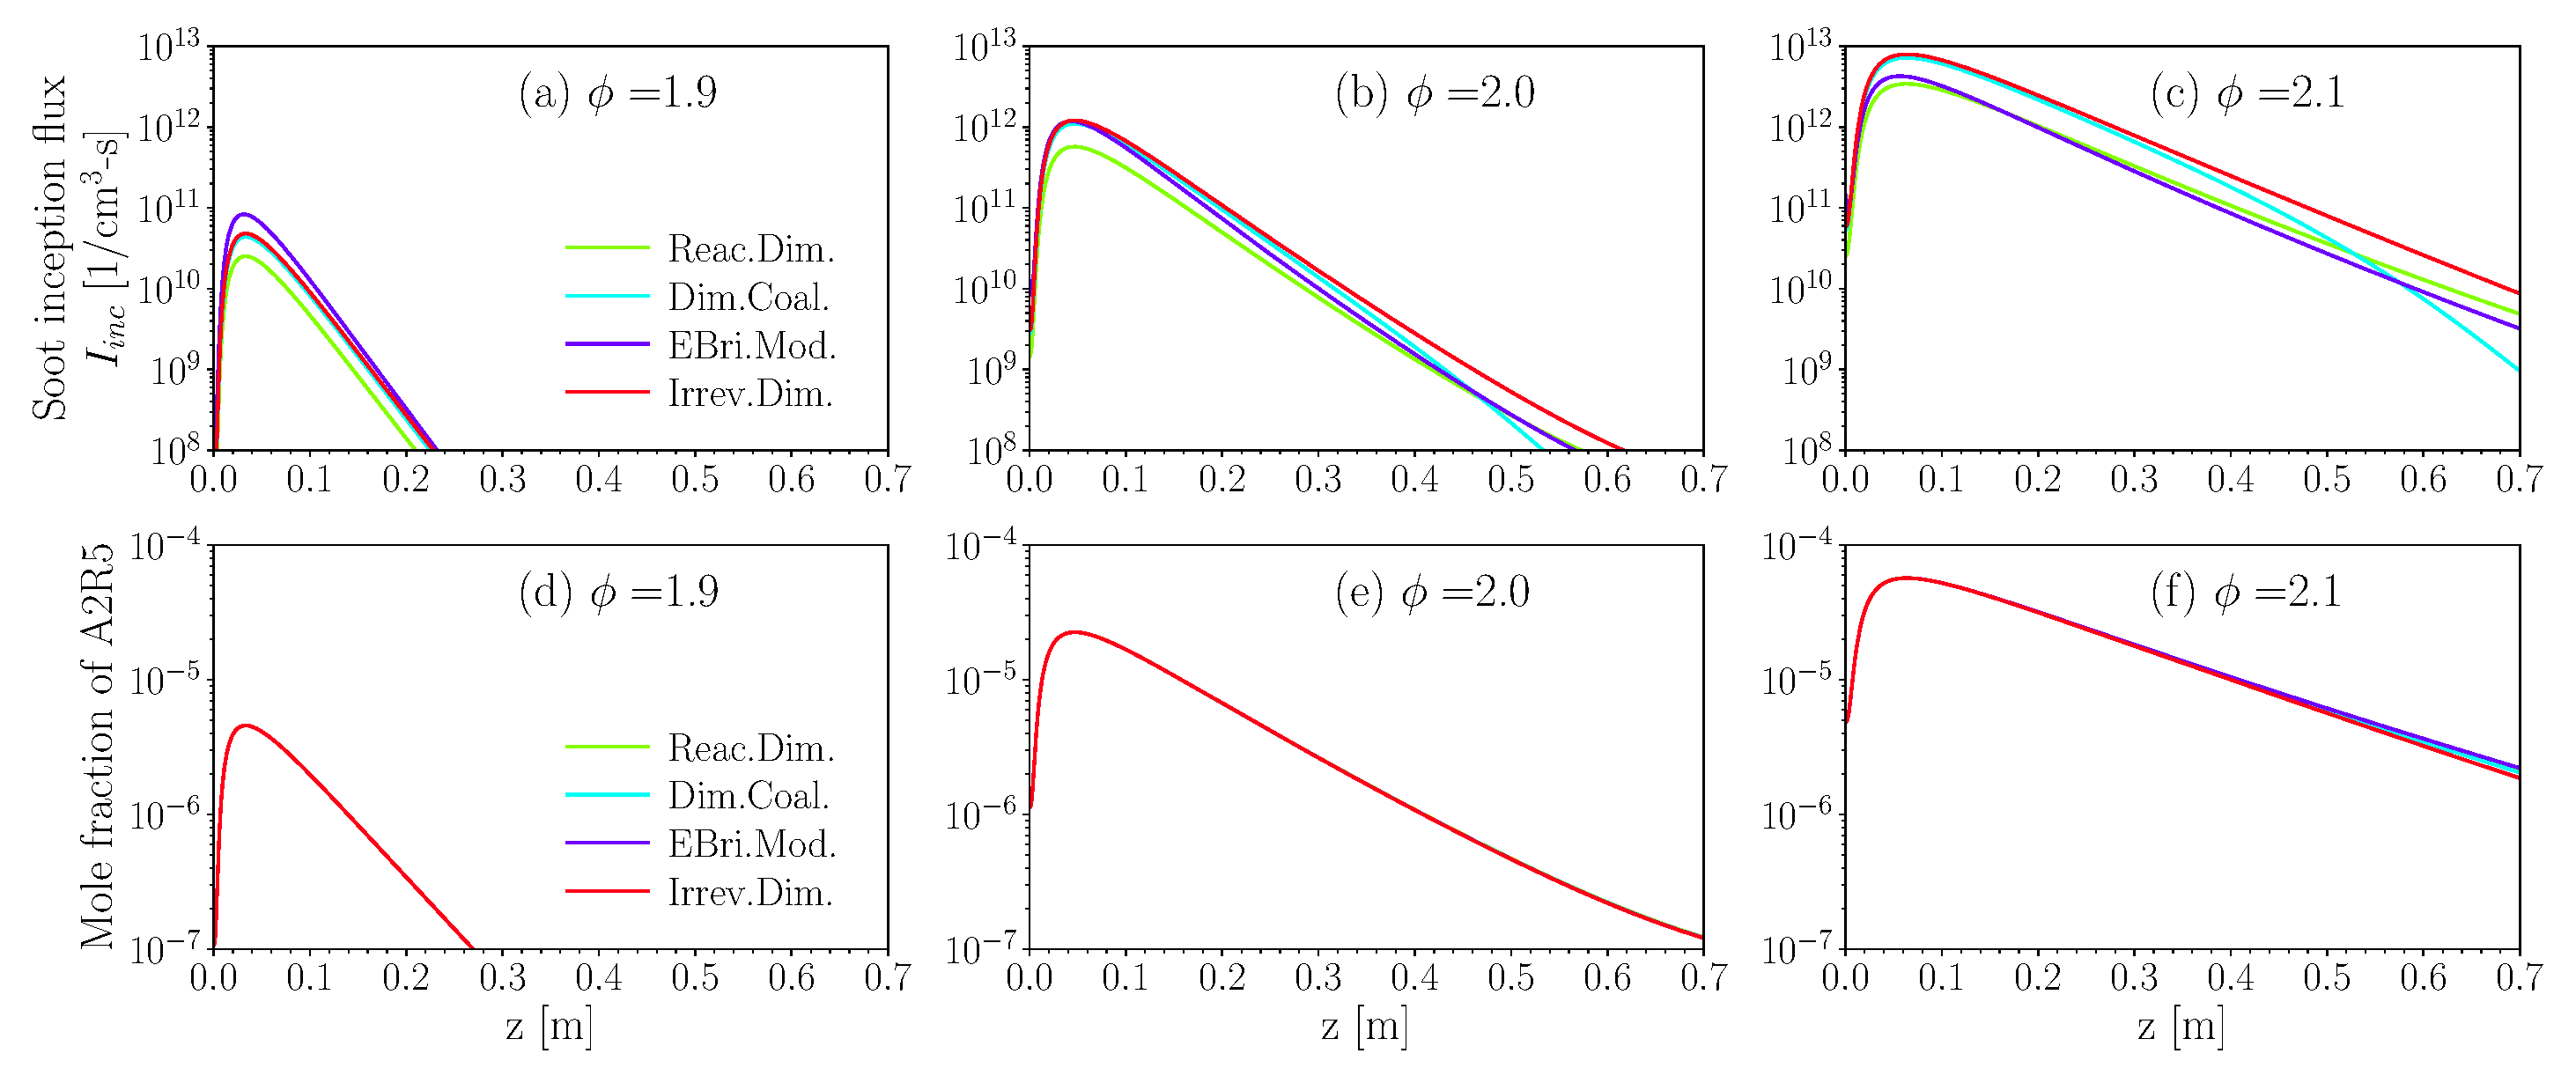
\includegraphics[width=1\textwidth]{Figures/Results/PSR/I_inc_PAH_eq_ratio_all_single_mech.pdf}
	\caption{The soot inception flux, $I_{inc}$ and acenaphthylene (A2R5) mole fraction along the PFR for $\phi=$1.9 (a,d), 2.0 (b,e), and 2.1 (c,f) obtained using KAUST mechanism, SPBM and different inception models calibrated to match the predictions with the PSD measurements~\citep{manzello2007soot}.}
	\label{fig:psrpfr_Iinc_PAH} 
\end{figure}

\begin{figure}[H]
	\centering
	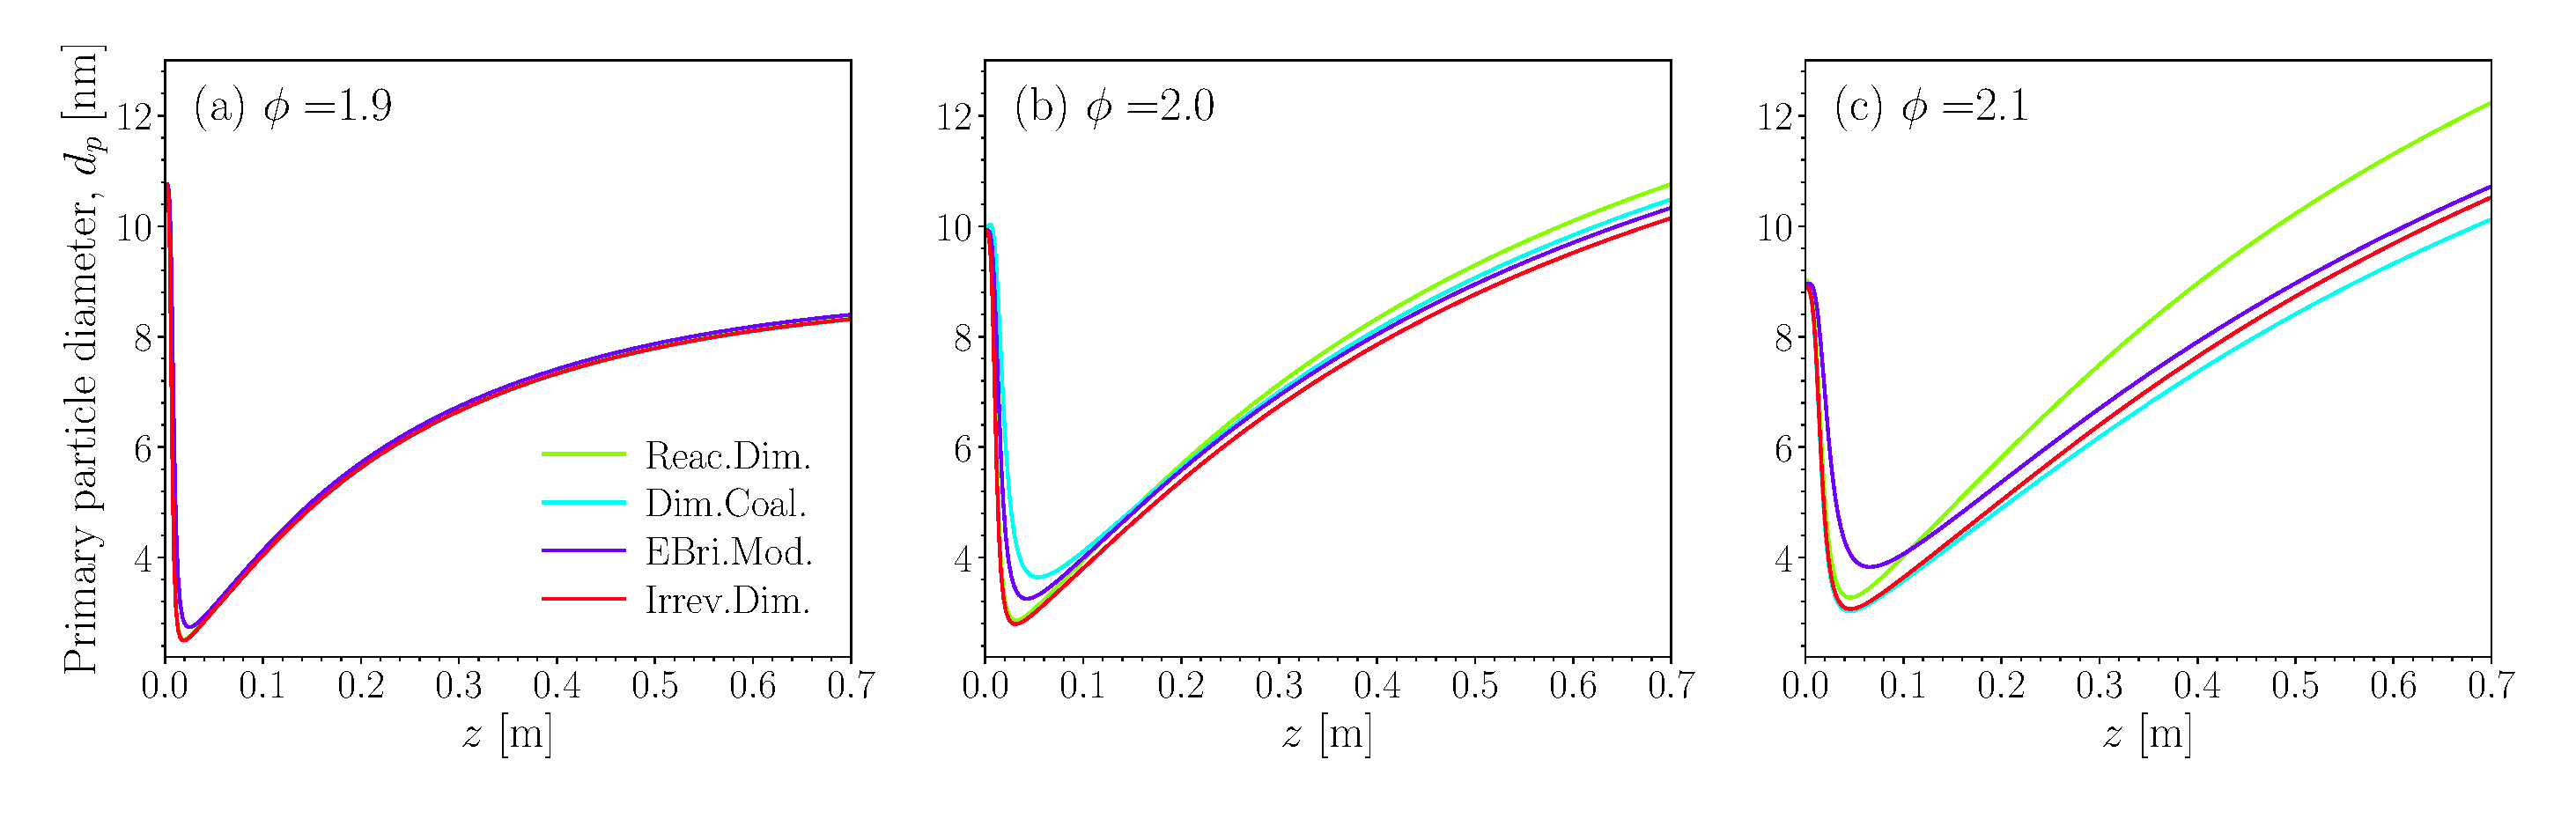
\includegraphics[width=1\textwidth]{Figures/Results/PSR/d_p_eq_ratio_all_single_mech.pdf}
	\caption{The primary particle diameter, $d_p$, along the PFR for $\phi$=1.9 (a), 2.0 (b), and 2.1 (c) obtained using KAUST mechanism, SPBM and different inception models calibrated to match the predictions with the PSD measurements~\citep{manzello2007soot}.}
	\label{fig:psrpfr_dp} 
\end{figure}

\begin{figure}[H]
	\centering
	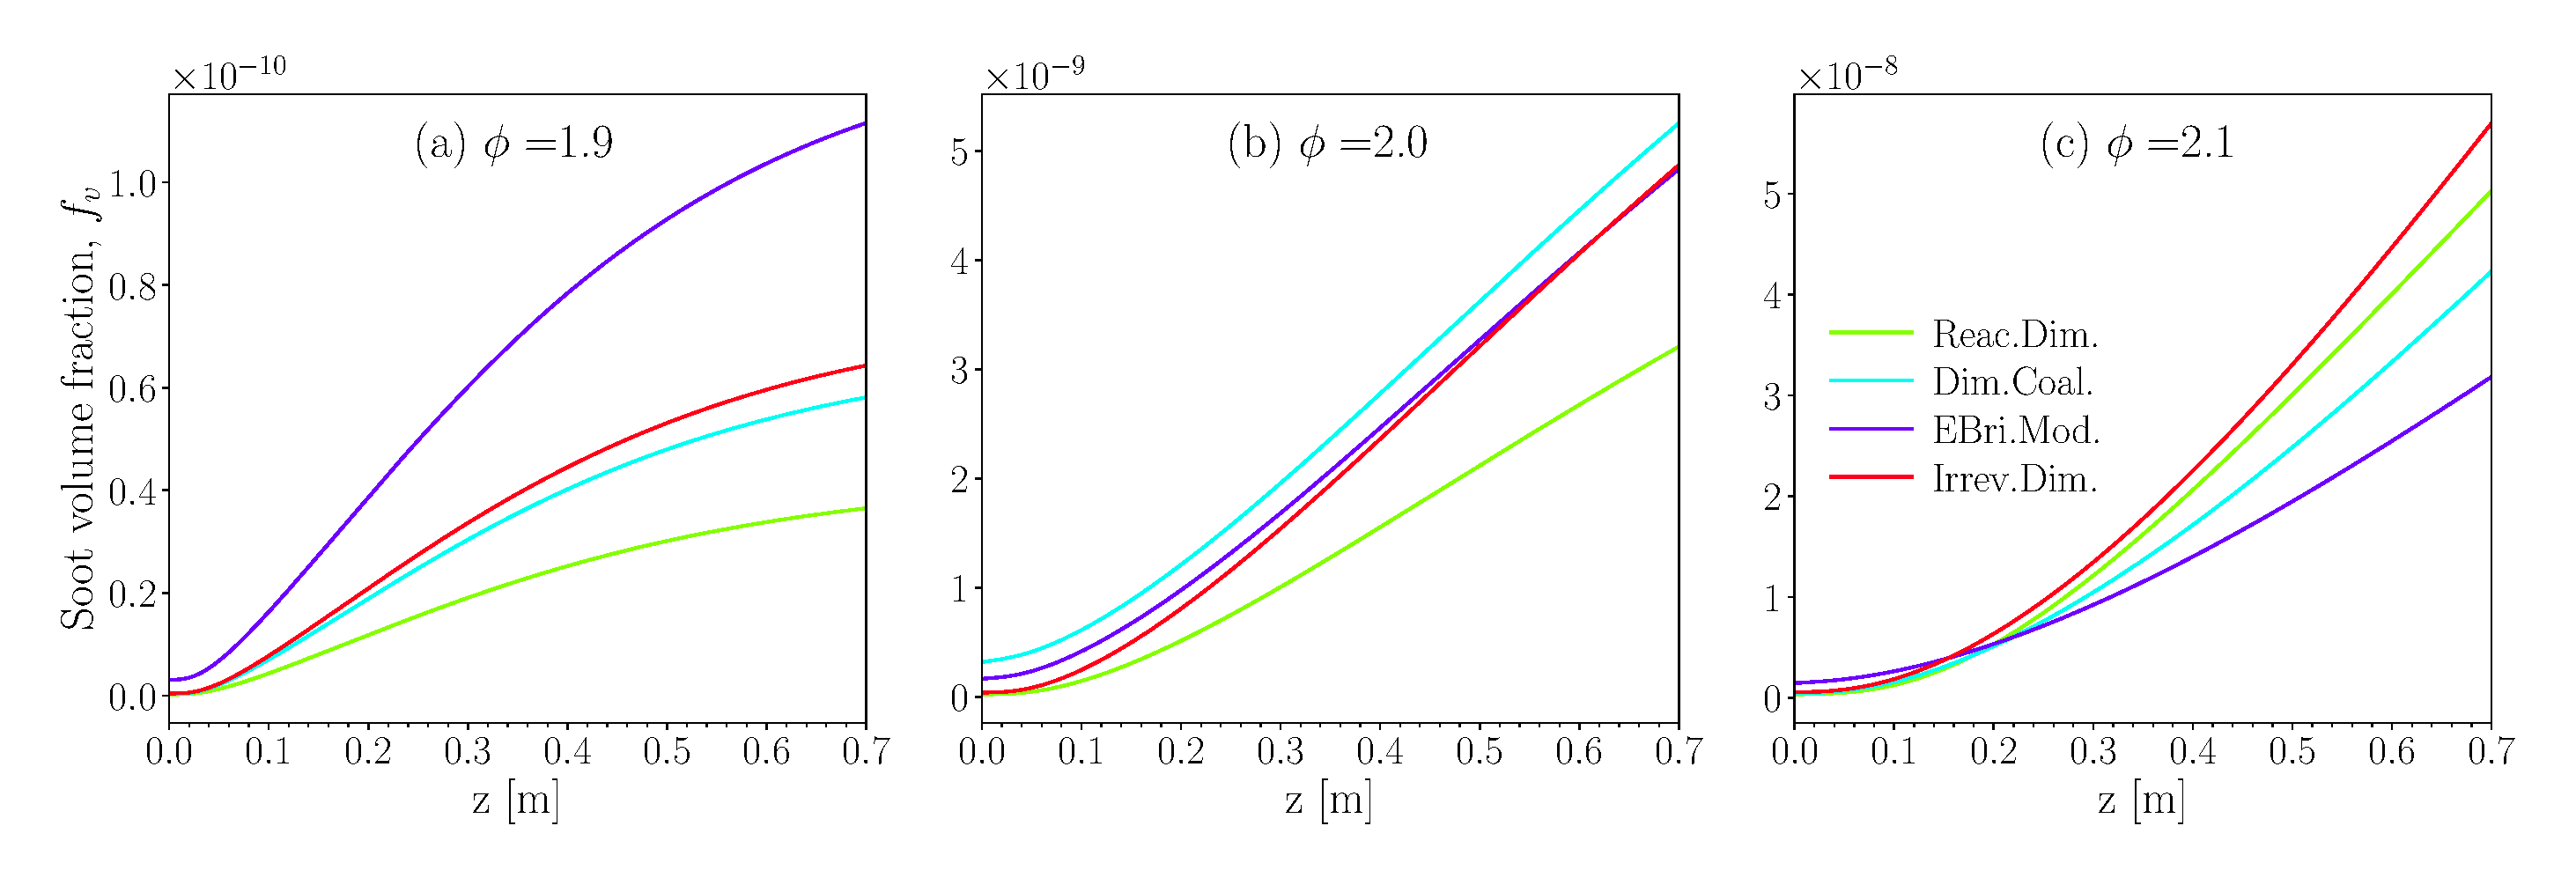
\includegraphics[width=1\textwidth]{Figures/Results/PSR/f_v_eq_ratio_all_single_mech.pdf}
	\caption{The soot volume fraction, $f_v$, along the PFR for $\phi=$1.9 (a), 2.0 (b), and 2.1 (c) obtained using KAUST mechanism and different inception models calibrated to match the predictions with the PSD measurements~\citep{manzello2007soot}.}
	\label{fig:psrpfr_fv} 
\end{figure}


